\documentclass[12pt, oneside]{article}
\usepackage{a4wide}
\usepackage{oldgerm}
\usepackage{amsmath}
\usepackage{amssymb}
\usepackage{amstext}
\setlength{\textheight}{8.875in} \setlength{\textwidth}{6.875in}
\setlength{\columnsep}{0.3125in} \setlength{\topmargin}{0in}
\setlength{\headheight}{0in} \setlength{\headsep}{0in}
\setlength{\parindent}{1pc} \setlength{\oddsidemargin}{-.304in}
\setlength{\evensidemargin}{-.304in}

%% Additional packages
\usepackage{enumitem}
\usepackage{tikz}
\usetikzlibrary{arrows,automata,positioning}
\usepackage{mathrsfs}

\begin{document}
\setlength{\textheight}{8.5in}
\centering {\bf MTL 106 (Introduction to Probability Theory and Stochastic Processes) }\\


\centering{\bf Assignment 2 Report}



\vskip 0.5cm

\noindent Name: Subhalingam D~~ ~~~  ~~~~~ ~~~~ ~~~~~~~~~~~~~~~~ Entry Number: 2018MT10770~~~~~~~~~~~



\vskip 0.5cm


\begin{enumerate}



\item Basic Probability

% Macro for sigma field notation
\newcommand{\sfield}[1] {$\mathscr{F}_{#1}$}
\newcommand{\sigmafield}{$\sigma$-field }

\textbf{\textit{Question:}}

Suppose there are three possible languages - English (E), Hindi (H) and Tamil (T) - a person can speak in a geographical area. We have $\Omega = \{E,H,T\}$. Find all possible \sigmafield that can be defined on $\Omega$. 
Let \sfield{1} be the second smallest (in terms of cardinality) $\sigma$-algebra defined on $\Omega$. To maintain uniqueness for solving further questions, we impose $\{T\} \in$ \sfield{1}. Let $P_1$ be a probability function defined on \sfield{1} such that $P_1(\{T\}) = 1/3$. Complete the function definition for $P_1$, i.e., find $P_1(X) \forall X \in $ \sfield{1}, if possible.

% Suppose there are three possible languages - English (E), Hindi (H) and Tamil (T) - a person can speak in a geographical area. We have $\Omega = \{E,F,H,T\}$. Find all possible \sigmafield defined on $\Omega$. 
% Let \sfield{1} be the second smallest (in terms of cardinality) $\sigma$-algebra defined on $\Omega$. To maintain uniqueness for solving further questions, we impose $\{T\} \in$ \sfield{1}. Let $P_1$ be a probability function defined on \sfield{1} such that $P_1(\{T\}) = 1/3$. Complete the function definition on $P_1$, i.e., find $P_1(X) \forall X \in $ \sfield{1}, if possible.


% Now consider \sfield{2}, another $\sigma$-algebra defined on $\Omega$. It is known that $\{T\}$ and $\{E\}$ belongs to \sfield{2}. Define another probability function $P_2$ on \sfield{2}. 


% Now consider \sfield{1}, \sfield{2} and \sfield{3} which are three $\sigma$-algebra defined on $\Omega$ such that \sfield{1} $\supset$ \sfield{2} $\supset$ \sfield{3}. To maintain uniqueness to solve further questions, we impose $\{T\} \in$ \sfield{2}. Let $P$ be a probability function defined on \sfield{2}. If $P(\{T\}) = \frac{1}{4}$, 

% $forall x \in$ \sfield{2}, find $P(x)$ that can be found where 

\textbf{\textit{Solution:}}

A \sigmafield \sfield{} has three properties:
\begin{enumerate}
    \item $\emptyset \in$ \sfield{} \\
    \item $A \in$ \sfield{} $\implies A^C \in$ \sfield{} \\
    \item For $A_i\in$\sfield{}, $\bigcup A_i \in $ \sfield{}
\end{enumerate}
An immediate corollary $\Omega\in$\sfield{} follows from (a) and (b).

So we have a trivial \sigmafield $\{\emptyset,\Omega\}$.

Next, we try to add one singleton to the \sigmafield. W.l.o.g., let $\{T\}$ belong to the \sigmafield and this implies $\{T\}^C = \{E,H\}$ should also belong to this \sigmafield. Their union is $\{E,H,T\} = \Omega$  which belongs to it already. So the next smallest \sigmafield possible are $\{\emptyset,\{E\},\{H,T\},\Omega\}$, $\{\emptyset,\{H\},\{E,T\},\Omega\}$ and $\{\emptyset,\{T\},\{E,H\},\Omega\}$.

Next we try to include two singletons, w.l.o.g. let them be $\{E\}$ and $\{H\}$. But if $\{E\}$ and $\{H\}$ belong to a \sigmafield, then their union $\{E,H\}$ should also belong to it and hence. $\{E,H\}^C = \{T\}$ should also belong to it. Hence, two singleton is not possible in our case.

For three elements, we can observe that the \sigmafield should be the power set of $\Omega$ which is $\{\emptyset,\{E\},\{H\},\{T\},\{E,H\},\{E,T\}, \{H,T\},\{E,H,T\}\}$

To summarize, the following five \sigmafield are possible:
\begin{enumerate}[label=(\roman*)]
\item $\{\emptyset,\Omega\}$ \\
\item $\{\emptyset,\{E\},\{H,T\},\Omega\}$ \\
\item $\{\emptyset,\{H\},\{E,T\},\Omega\}$ \\
\item $\{\emptyset,\{T\},\{E,H\},\Omega\}$
\item $\{\emptyset,\{E\},\{H\},\{T\},\{E,H\},\{E,T\}, \{H,T\},\Omega\}$

\end{enumerate}

The second smallest \sigmafield with $\{T\}$ is \sfield{1} $ = \{\emptyset,\{T\},\{E,H\},\Omega\}$. If $P_1$ is a probability function defined on \sfield{1}, it should follow \textbf{Kolmogrov's axioms of probability}. So, $P_1(\Omega) = 1$ and $P_1(\emptyset) = 0$. We have $P_1(\{T\}) = 1/3$ (given). Since $\{T\}$ and $\{E,H\}$ are disjoint and $\{T\} \cup \{E,H\} = \Omega$ and from Kolmogrov's third axiom of probability, $P_1(\{T\}) + P_1(\{E,H\}) = P_1(\Omega)$ and hence $P_1(\{E,H\}) = 1 - 1/3 = 2/3$

Hence we have 
\[ P_1(X) = 
\begin{cases}
0 & X = \emptyset \\
1/3 & X = \{T\} \\
2/3 & X = \{E,H\} \\
1 & X = \Omega
\end{cases}
\]

\newpage

\item Random Variable/Function of a Random Variable

\textbf{\textit{Question:}}

The cabs from a particular travels company arrive $X$ minutes late than the expected time of arrival where $X$ is a continuous rv uniformly distributed between 0 and 10 minutes. To attract customers, they add a discount of $R$ paise (1 paise = 0.01 rupees) where $R = e^{X+1}$. Suppose a customer books a cab, find the pdf for the discount he/she can get due to late arrival and the expected discount for the same?

\textbf{\textit{Solution:}}

The cdf of discount for late arrival is:
        \[\def\arraystretch{1.4}
            \begin{array}{lclr}
                F_R(r) & = & P(R \le r) & ~ \\
                ~ & = & P(e^{X+1} \le r) & \text{(Substituting }R\text{)} \\
                ~ & = & P(X \le \ln r - 1) & ~  \\
                ~ & = & \int_0^{\ln r - 1} \frac{1}{10} dx & ~  \\
                ~ & = & \frac{\ln r - 1}{10} & \text{for } e^1 \le r \le e^{11}
            \end{array}
        \]\\

The pdf can be found by differentiating the cdf and we obtain:
        \[ f_R(r) =
            \begin{cases}
                \frac{1}{10r}   & e^1 \le r \le e^{11} \\
                0               & \text{otherwise}
            \end{cases}
        \]

The expected discount could have been found without using the pdf of $R$ as $\int_0^{10} e^{x+1}f_X(x)dx$ but since we have found the pdf of $R$, we can directly write
        \[\def\arraystretch{1.4}
            \begin{array}{lcl}
                E(R) & = & \int_{e^1}^{e^{11}} r \frac{1}{10r} dr \\
                ~ & = & \frac{e^{11} - e^1}{10} \\
                ~ & \approx & 59.87 \text{ rupees}
            \end{array}
        \]\\


\newpage

\item Stochastic Processes

\textbf{\textit{Question:}}

Akash is determined to get an internship and starts mailing to companies continuously starting from time $t=0$. The time the mails are sent is a Poisson process with rate $\lambda_A$ per hour. Let $X$ denote time at which Akash sends his second mail. Bala who has been doing his assignments got inspired and motivated by Akash and starts sending the mails from $t=1$. The mails sent by Bala is also a Poisson process with rate $\lambda_B$ per hour and is independent of Akash. \textit{Note that all times mentioned in the time intervals are in hours.}

\begin{enumerate}[label=(\alph*)]

\item What is the probability that Akash sends exactly 5 mails during the time interval $[1,2]$?
\item You come at $t=1$ and got to know that Akash has sent one mail so far (and start doing some probability calculations). Find the conditional expectation of $X$ given this information?
\item What is the pmf of total number of mails sent by both Akash and Bala together during the time interval $[0,2]$?
% \item What is the expected time until each one of them have sent at least one email? (Note that mails sent by Akash during the interval $[0,1]$ should also be taken into account)
\item It is known that total 10 mails we sent by both of them in the time interval $[0,2]$. Find the probability that exactly 6 of them are sent by Akash? 

\end{enumerate}

\textbf{\textit{Solution:}}

\begin{enumerate}[label=(\alph*)]

\item The number of mails that Akash sends in time interval $[1,2]$ is rv with $Poisson(\lambda_A)$. So the probability that Akash sends exactly 5 mails during the time interval $[1,2]$ is $\frac{\lambda_A^5 e^{-\lambda_A}}{5!}$.

\item Let $A$ denote the event of exactly one arrival during the time interval $[0,1]$. From $t=1$, time until next arrival is an rv $T$ that is exponentially distributed with parameter $\lambda_A$. So, 
\[ E(X|A) = 1 + E(T) = 1 + \frac{1}{\lambda_A} \]

\item 
    Let $N$ be the total number of mails sent by Akash and Bala in $[0,2]$. Let us split the intervals into $[0,1]$ (the interval in which only Akash is sending mails) and  $[1,2]$ (the interval in which both of them send mails). 
    
    If $N_1$ is the total number of mails sent in $[0,1]$, then $N_1$ is a $Poisson(\lambda_A)$ rv.
    
    If $N_2$ is the total number of mails sent in  $[1,2]$, then $N_2$ is a $Poisson(\lambda_A+\lambda_B)$ rv which follows from the reproductive property of (independent) Poisson distribution.
    
    We have $N=N_1+N_2$. So $N \sim Poisson(2\lambda_A+\lambda_B)$ because $N_1$ and $N_2$ are independent and the sum follows from reproductive property. So the pmf of $N$ is 
    \[ p_N(n) = 
    \begin{cases}
    \frac{(2\lambda_A+\lambda_B)^ne^{-(2\lambda_A+\lambda_B)}}{n!} & n=0,1,2,3,\dots \\
    0 & \text{otherwise}
    \end{cases}
    \]

\item   For Akash sent 6 mails and 10 mails totally, we can claim that Bala has sent 4 mails in the interval. Also note that Bala starts sending mails only after $t=1$.
        \[\def\arraystretch{1.4}
            \begin{array}{lcl}
                P(\text{Akash sends 6 mails}|\text{10 mails sent totally}) & = & \frac{P(\text{Akash sends 6 mails}, \text{ 10 mails sent totally})}{P(\text{10 mails sent totally})} \\
                ~ & = & \frac{P(\text{Akash sends 6 mails}, \text{ Bala sends 4 mails})}{P(\text{10 mails sent totally})} \\
                ~ & = & \dfrac{\frac{(2\lambda_A)^6 e^{-2\lambda_A}}{6!} \cdot \frac{\lambda_B^4 e^{-\lambda_B}}{4!}} {\frac{(2\lambda_A+\lambda_B)^{10}e^{-(2\lambda_A+\lambda_B)}}{10!}} \\
                ~ & = & ^{10}C_6 \Big(\frac{2\lambda_A}{2\lambda_A+\lambda_B}\Big)^6 \Big(\frac{\lambda_B}{2\lambda_A+\lambda_B}\Big)^4
            \end{array}
        \]\\
        

\end{enumerate}

\newpage
\item Stochastic Processes

\textbf{\textit{Question:}}


%\begin{enumerate}[label=(\alph*)]

%\item
Consider a random process $X(t),t\in\mathbb{R}$ defined as
\[
X(t) = \sum_{j=-\infty}^{+\infty} A_jf_j(t)
\]
where $j\in\mathbb{Z}$; $A_j$s are iid rv with $E(A_j) = 1$ and $var(A_j) = 1$; $f_j(t)$ is defined as
\[ f_j(t) =
\begin{cases}
1 & j < t \le j+1 \\
0 & \text{otherwise}
\end{cases}
\]
% Classify the process as continuous-time or discrete-time.
Compute $E(X(t))$ and $E(X(t_1)X(t_2))$ for $t,t_1,t_2 \in \mathbb{R}$.

% \item Let $Y(t)$ be a continuous time WSS process such that  $E(X(t)) = 1$ and $E(X(t_1)X(t_2))$ 

%\item
%Let $T\in\mathbb{R}^+$ and rv $U \sim Uniform(0,T)$. Consider a real periodic function $p:\mathbb{R}\rightarrow\mathbb{R}$ with period $T$. Define random process $\{X(t), t \in \mathbb{R}$ as $X(t) = p(t+U)$ $\forall t \in \mathbb{R}$. Show that $X(t)$ is a WSS random process.

%\end{enumerate}

\textbf{\textit{Solution:}}


%\begin{enumerate}[label=(\alph*)]

%\item

        The given process is a continuous-time random process.
        
        It can be observed that for $j \in \mathbb{Z}$, $f_j(t)=0$ $\forall t \in \mathbb{R} \setminus (j,j+1]$. So for $t\in (j,j+1] $, $X(t) = A_j$.
        
        Hence, $E(X(t)) = E(A_j) = 1$ $\forall t \in \mathbb{R}$.
        
        Consider $t_1,t_2 \in \mathbb{R}$. There are two cases: these numbers can belong to the same interval or different interval. \textit{(Note that $A_j$s are iid rv is given)}.
        
        \textit{Case (i): } $j< t_1,t_2 \le j+1$,  then $E(X(t_1)X(t_2)) = E((A_j)(A_j)) = E((A_j)^2) = var(A_j) + E(A_j) = 1+1 = 2$.
        
        \textit{Case (2): } $j< t_1 \le j+1$ and $k< t_2 \le k+1$ where $j,k\in\mathbb{Z}$ and $j\ne k$, then $E(X(t_1)X(t_2)) = E((A_j)(A_k)) = E(A_j)E(A_k) = 1 \times 1 = 1$.

Hence, we have 
\[ E(X(t_1)X(t_2)) = 
\begin{cases}
2 & \text{if } t_1,t_2 \text{ belong to same sub-interval } (j,j+1] \text{ for } j \in \mathbb{Z} \\
1 & \text{if } t_1,t_2 \text{ belong to different sub-intervals }
\end{cases}
\]
  
% \item
%
%    If $p(t)$ is a periodic function defined on real domain, with period $T$, then $p(t+T) = p(t) \forall t \in \mathbb{R}$ by definition. 
%    
%    Let $t_1,t_2\in\mathbb{R}$, we can take $t_1 = t$ and $t_2 = t + \Delta t$ for $t,\Delta t\in\mathbb{R}$. Then, 
    
%        \[\def\arraystretch{1.4}
%            \begin{array}{lclr}
%               E(X(t_1)) - E(X(t_2)) & = & E(p(t_1+U)) - E(p(t_2+U)) \\
%               ~ & = & \int_{0}^{T} p(t_1+u)\cdot \frac{1}{T} du - \int_{0}^{T} p(t_2+u)\cdot \frac{1}{T} du \\
%               ~ & = & \int_{0}^{T} p(t_1+u)-p(\cdot \frac{1}{T} du
%            \end{array}
%       \]\\
    
    

%\end{enumerate}

\newpage
\item DTMC

\textbf{\textit{Question:}}

Consider DTMC $\{ X_n, n=0,1,2,\dots \}$ having states $\{1,2,3,\dots,9\}$ with the following state transition diagram given below. \textbf{Consider the initial state as $6$}, i.e., $P(X_0 = 6) = 1$ and give its transition probability matrix.

\begin{figure}[!h]
\centering
\begin{tikzpicture}[shorten >=1pt,node distance=2.5cm, auto]
  \node[state] (1)                {$1$};
  \node[state] (2) [right=of 1]   {$2$};
  \node[state] (3) [below=of 1]   {$3$};
  \node[state] (4) [below=of 2]   {$4$};
  \node[state] (5) [right=of 2]   {$5$};
  \node[state] (6) [below=of 5]   {$6$};
  \node[state] (7) [right=of 5]   {$7$};
  \node[state] (8) [below=of 7]   {$8$};
  \node[state] (9) [right=of 7]   {$9$};
  
  \path[->] (1) edge                node [above] {3/4} (2)
                edge [bend left]    node [left]  {1/4} (3)
            (2) edge [loop above]   node         {2/3} ()
                edge [bend left]    node [right] {1/3} (4)
            (3) edge [bend left]    node [left]  {1/2} (1)
                edge                node [above] {1/2} (4)
            (4) edge                node [above] {1/6} (1)
                edge [bend left]    node [right] {1/3} (2) 
                edge [bend left=45] node [below] {1/2} (3)
            (5) edge [bend left]    node [right]  {1/2} (6)
                edge                node [above] {1/2} (7)
            (6) edge                node [above] {1/2} (4)
                edge [bend left]    node [left]  {1/4} (5)
                edge                node [above] {1/4} (8)
            (7) edge [loop above]   node         {3/4} ()
                edge [bend left=45] node [above] {1/4} (9)
            (8) edge                node [left]  {1/3} (7)
                edge                node [left]  {2/3} (9)
            (9) edge                node [below] {1/4} (7)
                edge [bend left]    node [right] {1/4} (8)
                edge [loop above]   node         {1/2} ()
                
    ;
\end{tikzpicture}
\end{figure}

\begin{enumerate}[label=(\alph*)]
% \item Write down the Transition Matrix?
\item Find $P(X_2=7)$?
\item What is the steady-state probability of being in state $5$?
\item Find all the recurrent classes. Suppose $R_1$ be the smallest (least number of states within it) such recurrent class. Find the probability that the chain gets absorbed in $R_1$, if it exists?

% \item Suppose there are $N$ recurrent classes $R_1,R_2,\dots,R_N$ ordered such that $n(R_1) \le$ $n(R_2) \le \dots \le R_N$. Find $N$ and $R_i$s. \textit{For example, if there are three recurrent classes with two, three and four states; then $R_1$ is the class with two states, $R_2$ is the class with three states and $R_3$ is the class with four states.}
\end{enumerate}

\textbf{\textit{Solution:}}

The transition probability matrix $P$ is given by
\[ P = 
\begin{pmatrix}
0   & 3/4 & 1/4 & 0   & 0   & 0   & 0   & 0   & 0   \\
0   & 2/3 & 0   & 1/3 & 0   & 0   & 0   & 0   & 0   \\
1/2 & 0   & 0   & 1/2 & 0   & 0   & 0   & 0   & 0   \\
1/6 & 1/3 & 1/2 & 0   & 0   & 0   & 0   & 0   & 0   \\
0   & 0   & 0   & 0   & 0   & 1/2 & 1/2 & 0   & 0   \\
0   & 0   & 0   & 1/2 & 1/4 & 0   & 0   & 1/4 & 0   \\
0   & 0   & 0   & 0   & 0   & 0   & 3/4 & 0   & 1/4 \\
0   & 0   & 0   & 0   & 0   & 0   & 1/3 & 0   & 2/3 \\
0   & 0   & 0   & 0   & 0   & 0   & 1/4 & 1/4 & 1/2 \\
\end{pmatrix}
\]

\begin{enumerate}[label=(\alph*)]
\item 
        To reach $7$ from $6$ in two steps, there are two possible paths: $6\rightarrow8\rightarrow7$ and $6\rightarrow5\rightarrow7$ and hence,
        % $P(X_2=7,X_0=6) = P(X_2=7,X_1=8,X_0=6) + P(X_2=7,X_1=5,X_0=6) =  \frac 1 3 \cdot \frac 1 4 + \frac 1 2 \cdot \frac 1 4 = \frac{5}{24}$
        \[\def\arraystretch{1.4}
            \begin{array}{lcl}
            P(X_2=7,X_0=6) & = &  P(X_2=7,X_1=8,X_0=6) + P(X_2=7,X_1=5,X_0=6) \\
            ~ & = & \frac 1 3 \cdot \frac 1 4 + \frac 1 2 \cdot \frac 1 4 \\
            ~ & = & \frac{5}{24}
            \end{array}
        \]

\item State $5$ is transient. So the steady-state probability of being in state $5$ is $0$.

\item 
        There are two recurrent classes. The smallest one among them $R_1$ is $\{7,8,9\}$. The other one is $\{1,2,3,4\}$ (call it $R_2$).
        To obtain the probability that the chain gets absorbed in $R_1$, we will redraw the state diagram as:
        
        \begin{figure}[!h]
        \centering
        \begin{tikzpicture}[shorten >=1pt,node distance=2.5cm, auto]
          \node[state] (r2)[below=of 2]   {$R_2$};
          \node[state] (5) [right=of 2]   {$5$};
          \node[state] (6) [below=of 5]   {$6$};
          \node[state] (r1)[right=of 5]   {$R_1$};
          
          \path[->]
                    (5) edge [bend left]    node [left]  {1/2} (6)
                        edge                node [above] {1/2} (r1)
                    (6) edge                node [above] {1/2} (r2)
                        edge [bend left]    node [left]  {1/4} (5)
                        edge                node [above] {1/4} (r1)
            ;
        \end{tikzpicture}
        \end{figure}
        
        Now define $a_i = P(\text{absorption by }R_1 | X_0=i)$ $\forall i \in S'$ where $S'$ is the modified state space $\{R_1,R_2,5,6\}$. 
        
        We make use of this formula to obtain $a_i$:  \begin{align*}a_i = \sum_{j\in S} a_jP_{i,j}\end{align*}
        
        We set $a_{R_1} = 1$ and $a_{R_2} = 0$ according to requirement of the question. We obtain $a_5$ and $a_6$ by solving:
        \[\def\arraystretch{1.4}
            \begin{array}{lcl}
            a_5 & = & \frac 1 2 \cdot a_{R_1} + \frac 1 2 \cdot a_{6} + 0 \cdot a_{R_2} \\
            ~ & = & \frac 1 2 + \frac 1 2 \cdot a_{6} \\
            
            a_6 & = & \frac 1 4 \cdot a_{R_1} + \frac 1 4 \cdot a_{5} + \frac 1 2 \cdot a_{R_2} \\
            ~ & = & \frac 1 4 + \frac 1 4 \cdot a_{5}
            \end{array}
        \]
        
        Solving the equations we have $a_5 = \frac 5 7$ and $a_6 = \frac 3 7$
        
        Hence, the probability that the chain gets absorbed in $R_1$ if initially started from state $6$ is $a_6 = \frac 3 7$
        
\end{enumerate}

\newpage
\item DTMC

\textbf{\textit{Question:}}

Consider a language in which a character can belong to any of the following three (exhaustive) types - consonants, vowels and white spaces. Assume that other symbols are included in one of vowels or consonants as we are not interested in them. In this language, the type of next character depends only on the present character (in short, it follows Markov Property). The white space are used to mark (differentiate between) two different words \textit{and are the only markers to differentiate two words}. Also, there is no white space in the beginning and at the end of text and there are NO extra (two adjacent) white spaces in the corpus. Given a vowel, the probability that the next character is also vowel is $1/3$ and the next character is a consonant is $1/2$. Given a consonant, the probability that the next character is also a consonant is $2/5$ and a vowel is $2/5$. The probability that a word begins with a consonant is $2/3$. 

The above model can be modelled as DTMC. Complete the transition state diagram and answer the following questions:
\begin{enumerate}[label=(\alph*)]
\item Find the expected number of \textbf{words} in a corpus with 115 million characters?
\item Find the long-run average rate of transitions from a vowel to consonant in the same corpus with 115 million characters?

\end{enumerate}

\textbf{\textit{Solution:}}

Consider DTMC $\{ X_n, n=0,1,2,\dots \}$ having states $\{V,C,S\}$ where $V$, $C$, $S$ represent vowel, consonant and white-space respectively.

From the description, we get the transition probability matrix $P$ (in the order $(C,V,S)$ as:
\[ P = 
\begin{pmatrix}
1/3    & 1/2    & p_{13} \\
2/5    & 2/5    & p_{23} \\
p_{31} & p_{32} & p_{33} \\
\end{pmatrix}
\]

We make the following observations:
\begin{itemize}
    \item $p_{33} = 0$ as two white-spaces can't occur be adjacent to each other \textit{(given)}
    \item $p_{32} = 2/3$ as the probability that a word begins with a consonant \textit{(which means transition from white-space to consonant)} is $2/3$ \textit{(given)}
    \item $p_{13} = 1/6$, $p_{23} = 1/5$ and $p_{31} = 1/3$ as the sum of probabilities in a row should add up to one in $P$
\end{itemize}

Now, we complete the transition probability matrix $P$ as
\[ P = 
\begin{pmatrix}
1/3    & 1/2    & 1/6    \\
2/5    & 2/5    & 1/5    \\
1/3    & 2/3    & 0      \\
\end{pmatrix}
\]

And hence, we can draw the following state transition diagram:
        \begin{figure}[!h]
        \centering
        \begin{tikzpicture}[shorten >=1pt,node distance=2.5cm, auto]
          \node[state] (V)                {$V$};
          \node[state] (C) [right=of V]   {$C$};
          \node[state] (S) [below=of C]  {$S$};

          \path[->]
                    (V) edge [loop above]   node         {1/3} ()
                        edge [bend left]    node [above] {1/2} (C)
                        edge [bend right]   node [left] {1/6} (S)
                    (C) edge                node [below] {2/5} (V)
                        edge [loop above]   node         {2/5} ()
                        edge [bend left]    node [right] {1/5} (S)
                    (S) edge                node [below] {1/3} (V)
                        edge     node [left]  {2/3} (C)
            ;
        \end{tikzpicture}
        \end{figure}

Moreover, we have the initial distribution as $X_0=\begin{pmatrix} 1/3 & 2/3 & 0 \end{pmatrix}$.

% We obtain the following state transition diagram:

To find the stationary distribution $\pi = \begin{pmatrix} \pi_V & \pi_C & \pi_S \end{pmatrix}$, we set up:

\[ \pi = \begin{pmatrix} \pi_V & \pi_C & \pi_S \end{pmatrix} = 
\begin{pmatrix} \pi_V & \pi_C & \pi_S \end{pmatrix}
\begin{pmatrix}
1/3    & 1/2    & 1/6    \\
2/5    & 2/5    & 1/5    \\
1/3    & 2/3    & 0      \\
\end{pmatrix}
\]
where we get the following equations:
        \[\def\arraystretch{1.4}
            \begin{array}{lcl}
            \pi_V & = & \frac{\pi_V}{3} + \frac{2\pi_C}{5} + \frac{\pi_S}{3} \\
            \pi_C & = & \frac{\pi_V}{2} + \frac{2\pi_C}{5} + \frac{2\pi_S}{3} \\
            \pi_S & = & \frac{\pi_V}{6} + \frac{\pi_C}{5} + 0 \\
            1 & = & \pi_V + \pi_C + \pi_S \\
            \end{array}
        \]
Upon solving, we get $\pi = \begin{pmatrix} 42/115 & 55/115 & 18/115 \end{pmatrix}$

We can make the following observations on the chain:
\begin{itemize}
    \item \textbf{irreducible} as we can go from one state to any other state in finite number of steps
    \item \textbf{aperiodic} as there is a self-transition (e.g. $p_{11} > 0$)
    \item all states are \textbf{+ve recurrent} as it is a finite state space irreducible DTMC
\end{itemize}
\textbf{Hence, the limiting distribution exists and is equal to the stationary distribution.}

\begin{enumerate}[label=(\alph*)]
\item The average fraction of characters that are white-spaces is $\pi_S = 18/115$. So the expected number of white-spaces is $\pi_S \cdot 115,000,000 = 18,000,000$. Expected number of words is one more than expected number of white-spaces and so that is $18,000,001$.

\item The long-run average rate of transitions from a vowel to consonant is $\pi_V \cdot p_{12} = \frac{42}{115}\cdot\frac{1}{2} = \frac{21}{115}$. So the expected number of such transitions will be $\frac{21}{115} \cdot 115,000,000 = 21,000,000$

\end{enumerate}

\newpage
\item CTMC

\textbf{\textit{Question:}}
Consider a CTMC $X(t)$ whose jump chain is given below:

        \begin{figure}[!h]
        \centering
        \begin{tikzpicture}[shorten >=1pt,node distance=2.5cm, auto]
          \node[state] (1)                {$1$};
          \node[state] (2) [right=of 1]   {$2$};
          \node[state] (3) [below=of 2]   {$3$};

          \path[->]
                    (1) edge [bend left]    node [above] {1/2} (2)
                        edge [bend right]   node [left]  {1/2} (3)
                    (2) edge                node [below] {3/4} (1)
                        edge                node [right] {1/4} (3)
                    (3) edge                node [right] {1}   (1)
            ;
        \end{tikzpicture}
        \end{figure}
Take $\lambda_1 = 1$, $\lambda_2 = 2$ and $\lambda_3 = 3$. Find the generator matrix for the chain and \textit{hence} find the limiting distribution for $X(t)$.
% Also state the Kolmogorov forward equation

\textbf{\textit{Solution:}}
The jump chain is irreducible and transition matrix for the jump chain is given by 
\[ P = 
\begin{pmatrix}
0       & 1/2   & 1/2    \\
3/4     & 0     & 1/4    \\
1       & 0     & 0      \\
\end{pmatrix}
\]

If the generator matrix $Q=(q_{ij})$, then 
\[ q_{ij}=
\begin{cases}
\lambda_i p_{ij} & i \ne j \\
- \lambda_i & i=j
\end{cases}
\]

We have $\lambda_1 = 1$, $\lambda_2 = 2$ and $\lambda_3 = 3$. Hence we can obtain the generator matrix as 
\[ Q = 
\begin{pmatrix}
-1      & 1/2   & 1/2    \\
3/2     & -2    & 1/2    \\
3       & 0     & -3      \\
\end{pmatrix}
\]

We can obtain the limiting distribution $\pi = \begin{pmatrix} \pi_1 & \pi_2 & \pi_3 \end{pmatrix}$ using the relation $\mathbf{\pi Q = 0}$ and having $\pi_1 + \pi_2 + \pi_3 = 1$ additionally. 

We obtain the following equations:
        \[\def\arraystretch{1.4}
            \begin{array}{lcl}
            -\pi_1 + \frac32\pi_2 + 3\pi_3 & = & 0 \\
            \frac12\pi_1 -2\pi_2 & = & 0 \\
            \frac12\pi_1 + \frac12\pi_2 -3 \pi_3 & = & 0 \\
            \pi_1 + \pi_2 + \pi_3 & = & 1 \\
            \end{array}
        \]

Solving the above equations, we get the limiting distribution for $X(t)$ as $\begin{pmatrix} \frac{24}{35} & \frac{6}{35} & \frac{5}{35} \end{pmatrix}$.



\newpage
\item CTMC

\textbf{\textit{Question:}}

The attendance for a course has to be marked through an online system. An app can be installed in the phones of the students to mark it directly from their phones and one tablet is installed in the room to assist students without a smartphone or for marking attendance in case of technical problems. One day, there is an update to the app which leads to a bug and not everyone is able to mark the attendance through their phones at once (in one attempt). So everyone decide to form a queue to mark the attendance in the tablet and standing in the queue, they also try to mark their attendance through their phones simultaneously to try their luck. Assume that all the students in the class have a smartphone (and the reason for queue is only because of technical difficulties) and for the sake of simplicity, also assume that the total number of students is not known and very large.

Students arrive to the tablet at rate of 15 per minute. On average, it takes about 30 seconds on average for a student to mark the attendance in the tablet which is exponentially distributed. \textit{However, if the student has successfully marked the attendance through mobile app while standing in line, he/she leaves the line immediately.} Suppose that the success for marking attendance in mobile app is exponentially distributed with average 2 minutes. 

Now, answer the following questions:
\begin{enumerate}[label=(\alph*)]
\item Draw the transition diagram and set up the equations for computing $\pi_i$s. \textit{It is not necessary to solve them and further questions can be answered in terms of $\pi_i$s.}

\item What is the long-run fraction of time that the tablet is occupied?
\item What fraction of students standing in the queue end up marking the attendance in their own phones, without ever reaching the tablet?
\item What fraction of students come for marking in the tablet and immediately mark their attendance in the tablet (without waiting in a queue)?
\end{enumerate}

\textbf{\textit{Solution:}}

\begin{enumerate}[label=(\alph*)]
\item

Let $X(t)$ be the number of students in the queue (both waiting and using the tablet). It can be claimed that $X(t)$ is a CTMC with state space $S=\{0,1,2,3,...\}$.

The arrival time to the system is $\lambda = 15$ per minute. However, for the departure, there are two possible cases: a student marking the attendance in the tablet (obtaining service) leaves after marking in the tablet, which happens with parameter $\mu_1 = 2$ per minute (as mean time taken is 30 seconds); or, a student waiting in the queue has successfully marked the attendance through the mobile app with parameter $\mu_2 = 0.5$ per minute (as mean time taken is 2 minutes).

For $i>1$ number of students in system, transition to next state ($i+1$) happens at a rate of $\lambda = 15$ per minute and the total rate for transition to previous state is $\mu = \mu_1 + (i-1)\cdot\mu_2$ as each of $(i-1)$ students in the queue (without service) has rate $\mu_2$ for leaving the queue and the person in service has rate $\mu_1$. Hence, $\mu = 2 + (i-1)0.5$ per minute.

Hence, we obtain the following state diagram:

\begin{figure}[!h]
\centering
\begin{tikzpicture}[shorten >=1pt,node distance=1.75cm, auto]
  \node[state] (0)                {$0$};
  \node[state] (1) [right=of 0]   {$1$};
  \node[state] (2) [right=of 1]   {$2$};
  \node[state] (3) [right=of 2]   {$3$};
  \node[state] (4) [right=of 3]   {$3$};
  \node[]     (inf)[right=of 4]   {$\mathbf{\cdots}$};
  
  \path[->]
            (0) edge [bend left]    node [above] {15} (1)
            (1) edge [bend left]    node [above] {15} (2)
                edge [bend left]    node [below] {2+0(0.5)}  (0)
            (2) edge [bend left]    node [above] {15} (3)
                edge [bend left]    node [below] {2+1(0.5)}  (1)
            (3) edge [bend left]    node [above] {15} (4)
                edge [bend left]    node [below] {2+2(0.5)}  (2)
            (4) edge [bend left]    node [above] {15} (inf)
                edge [bend left]    node [below] {2+3(0.5)}  (3)
            (inf)edge [bend left]   node [below] {2+4(0.5)}  (4)
    ;
\end{tikzpicture}
\end{figure}

With flow out equals flow in, we use balance equations to obtain $\pi_i$s.

\[\def\arraystretch{1.4}
    \begin{array}{rcl}
       15 \pi_0 & = & 2 \pi_1 \\
       (15 + 2)\pi_1 & = & 15 \pi_0 + (2+0.5) \pi_2 \\
       (15 + (2 + 1 \times 0.5))\pi_2 & = & 15 \pi_1 + (2+2 \times 0.5) \pi_3 \\
       (15 + (2 + 2 \times 0.5))\pi_3 & = & 15 \pi_2 + (2+3 \times 0.5) \pi_4 \\
       (15 + (2 + 3 \times 0.5))\pi_4 & = & 15 \pi_3 + (2+4 \times 0.5) \pi_5 \\
       \dots & = & \dots\\
       (15 + (2 + (i-1) \times 0.5))\pi_i & = & 15 \pi_{i-1} + (2+i \times 0.5) \pi_{i+1} \\
       \dots & = & \dots\\
       1 & = & \pi_0 + \pi_1 + \pi_2 \dots
    \end{array}
\]\\



\item The tablet is occupied if $X(t) \ge 1$ or $X(t) \ne 0$. Thus the the fraction of time that the tablet is occupied is $1-\pi_0$.

\item 
Students leave the queue after marking their attendance in their own phone at rate $(0) \pi_0 + (0) \pi_1 +(0.5) \pi_2 + (2 \times 0.5) \pi_3 +(3 \times 0.5) \pi_4 + \dots$ per minute and students arrive at rate of $15$ per minute. So fraction of students end up marking the attendance in their own phones, without ever reaching the tablet is $\frac{\pi_2 + 2\pi_3 + 3\pi_4 + 4\pi_5 + \dots}{30}$

\item Student coming at state $X(0) = 0$ can directly mark the attendance in the tablet without waiting. Thus the fraction of students come for marking in the tablet and immediately mark their attendance in the tablet (without waiting in a queue) is $\pi_0$.

\end{enumerate}



\newpage
\item Queueing Models

\textbf{\textit{Question:}}

\begin{enumerate}[label=(\alph*)]
\item 
        Consider a communication node in which packets arrive according to Poisson process. It has only one output link. Consider the following three cases and give Kendall notation for each of them:
        
        \begin{enumerate}[label=(\roman*)]
            \item Packets are exponentially distributed. The node has infinite buffer capacity.
            \item Packet length can be $l_1$, $l_2$, $l_3$, $l_4$, $l_5$ with probability $P_{l_1}$, $P_{l_2}$, $P_{l_3}$, $P_{l_4}$, $P_{l_5}$ respectively. The node has NO buffer capacity.
            \item Packet length is fixed, say $L$. The node has buffer capacity as $n$, i.e., only $n$ packets can be stored in the buffer.
        \end{enumerate}
\item 
        Consider M/M/106/4040/2020 and M/M/106/2020/2020 queuing system. Which one has better performance? Which one might you NOT prefer? Why/Why not?

\item
        Consider a pure delay process where customers arrive according to Poisson process with parameter $\lambda = 5$. The service time is an exponential distribution with mean $1/5$ minutes. There are two servers but only one of them is always available. The other server would, however, start the service only when the queue length becomes two. When there are no more customers in the queue, the server that becomes idle (complete service) first becomes unavailable for further service and remain unavailable until the queue length becomes two again. Take the discipline to be FCFS. Sketch the state diagram for this system?

% \item   
%        Consider a Internet Service Provider with four dial-up connections
\end{enumerate}

\textbf{\textit{Solution:}}

\begin{enumerate}[label=(\alph*)]

\item
        In all the cases,\\
        ~~ Arrival of packets is Poisson distribution - [M] \\
        ~~ Only one output link, meaning single server - [1] \\
        
        \begin{enumerate}[label=(\roman*)]
            \item Packets are exponentially distributed - [M] \\ Infinite buffer capacity \\
            So it is \textbf{M/M/1} system.
            \item Packet length can be $l_1$, $l_2$, $l_3$, $l_4$, $l_5$ with probability $P_{l_1}$, $P_{l_2}$, $P_{l_3}$, $P_{l_4}$, $P_{l_5}$ respectively which means general service - [G] \\
            No buffer capacity - [1] \\
            So it is \textbf{M/G/1/1} system.
            \item Packet length is fixed, meaning deterministic service - [D] \\
            Buffer capacity is $n$ + $1$ can be in service - [n+1] \\
            So it is \textbf{M/D/1/n+1} system.
        \end{enumerate}

\item
        Both M/M/106/4040/2020 and M/M/106/2020/2020 have same performance as customers fit into each system. However, M/M/106/4040/2020 might not be preferred because of wastage of buffer capacity. 

\item
        To summarize, we have Poisson arrivals, Exponential service time, 2 servers and infinite buffer. Suppose we denote the states by $S_{ij}$ where $i$ is the number of available (active) servers and $j$ is the total number of customers in system (waiting and in service). 
        
        By understanding the working of the system, we can note that there would be a transition from $S_{12}$ to $S_{23}$ as this is a case of arrival in which queue length becomes two, the server who was idle also starts working. Also, $S_{22}$ makes a transition to $S_{11}$ when a customer leaves and the other server has no more customers to serve and remains unavailable until the queue length becomes two again.
        
        We can now draw the following state transition diagram:
        
        \begin{figure}[!h]
        \centering
        \begin{tikzpicture}[shorten >=1pt,node distance=1.75cm, auto]
          \node[state] (s10)                {$S_{10}$};
          \node[state] (s11) [right=of s10]   {$S_{11}$};
          \node[state] (s12) [right=of s11]   {$S_{12}$};
          \node[state] (s22) [above=of s11]   {$S_{22}$};
          \node[state] (s23) [above=of s12 ]   {$S_{23}$};
          \node[state] (s24) [right=of s23]   {$S_{24}$};
          \node[state] (s25) [right=of s24]   {$S_{25}$};
          \node[]     (inf)  [right=of s25]   {$\mathbf{\cdots}$};
          
          \path[->]
                    (s10) edge [bend left]    node [above] {$5$} (s11)
                    (s11) edge [bend left]    node [above] {$5$} (s12)
                          edge [bend left]    node [below] {$5$} (s10)
                    (s12) edge [bend right]   node [left]  {$5$} (s23)
                          edge [bend left]    node [below] {$5$} (s11) 
                    (s22) edge [bend left]    node [above] {$5$} (s23)
                          edge [bend right]   node [right] {$2\times5$} (s11)
                    (s23) edge [bend left]    node [above] {$5$} (s24)
                          edge [bend left]    node [below] {$2\times5$} (s22)
                    (s24) edge [bend left]    node [above] {$5$} (s25)
                          edge [bend left]    node [below] {$2\times5$} (s23)
                    (s25) edge [bend left]    node [above] {$5$} (inf)
                          edge [bend left]    node [below] {$2\times5$} (s24)
                    (inf) edge [bend left]    node [below] {$2\times5$} (s25)
            ;
        \end{tikzpicture}
        \end{figure}

\end{enumerate}




\newpage
\item Queueing Models

\textbf{\textit{Question:}}

Consider a queuing system in front of counter of shop in which inter-arrival times of customers are modelled as Exponential Distribution with mean 50s. Consider the following three cases:
\begin{enumerate}[label=(\Alph*)]
    \item There is only one single-server queue. The service time is exponentially distributed with mean 40s. There is infinite buffer space.
    \item The owner hires two severs with average time of service for each server double that of case A (i.e., service time of each server is exponentially distributed with expectation 80s) to reduce the amount paid to servers. Two single-server queues are set up each with infinite buffer space.
    \item Consider the same two set of servers in Case (B) (i.e., service time of each server is exponentially distributed with expectation 80s). Instead of two single-server queue, one two-server queue is now set up with infinite buffer space.
\end{enumerate}
With the above three cases, answer the following questions:
\begin{enumerate}[label=(\roman*)]
\item Give the Kendall notations and the parameters of the distributions (inter-arrival and service) for each of the three cases?
\item What is the average number of customers in the system in cases (A) and (B)?
\item How long on average does each customer spend in the line \textbf{waiting to get served} in cases (A) and (B)?
% \item Find the response time in case (C)?
\end{enumerate}
\textit{(You can assume that a customer choosing a particular queue is equally likely in case (B))}



\textbf{\textit{Solution:}}

Let the parameter for inter-arrival time distribution of customers be $\lambda$ and the parameter for service time distribution be $\mu$.

\begin{enumerate}[label=(\roman*)]
\item   
        Case (A) is M/M/1 queue with $\lambda_A = 1/50 = 0.02$ and $\mu_A = 1/40 = 0.025$ \\
        Case (B) is effectively two M/M/1 queues. Since a customer joining a particular line is equally likely, the average inter-arrival time of customers would be double for a particular queue. So $\lambda_B = 1/100 = 0.01$ and $\mu_B = 1/80 = 0.0125$ \\
        Case (C) is M/M/2 queue. $\lambda_C = 1/50 = 0.02$ and $\mu_C = 1/80 = 0.0125$.

\item 
        Suppose $N$ represent number of customers in system, $R$ represent time spent and $Q$ be time spent in the line excluding the time spent for service.
        
        For M/M/1 queue,
        
        \[\def\arraystretch{1.4}
            \begin{array}{lclr}
                E(N) & = & \frac{\lambda}{\mu-\lambda} & ~ \\
                \lambda \cdot E(R) & = & E(N) & \text{(by Little's formula)} \\ 
                E(R) & = & \frac{1}{\lambda} \frac{\lambda}{\mu-\lambda} & ~ \\
                ~ & = & \frac{1}{\mu-\lambda} & ~ \\
                E(Q) & = & E(R) - \frac{1}{\mu} & ~ \\
                ~ & = & \frac{1}{\mu-\lambda} - \frac{1}{\mu} & ~
            \end{array}
        \]\\
        
        Using the above results we have the average number of customers in the system in case (A) as $\frac{\lambda_A}{\mu_A-\lambda_A} = \frac{0.02}{0.025-0.02} = 4$. For case (B), the average number of customers in each system is $\frac{\lambda_B}{\mu_B-\lambda_B} = \frac{0.01}{0.0125-0.01} = 4$. There are two such systems and totally, $8$ customers are expected in the both the systems for the counter.
        
\item   
        The average time spent in the line excluding the time spent for service by each customers in case (A) is $\frac{1}{\mu_A-\lambda_A} - \frac{1}{\mu_A} = \frac{1}{0.025-0.02} - \frac{1}{0.025} = 160s$ and in case (B), it is $\frac{1}{\mu_B-\lambda_B} - \frac{1}{\mu_B} = \frac{1}{0.0125-0.01} - \frac{1}{0.0125} = 320s$.

%\item
%        We have $\rho = \frac{\lambda_C}{2\mu_C} = 0.8$.
%        For a 

        
\end{enumerate}

\end{enumerate}

\end{document}
